\section{Limit Checks and the truncation label}\label{sec:9.4}

The free-recoil formula $\omega = q^2/2M$ holds for a silicon nucleus once the recoil energy exceeds nine phonon energies, \SI{0.54}{eV} for a nucleus in an Einstein well of \SI{60}{meV}. \Cref{lim:1.3a} showed this with one plot: the formula against the bound nucleus, the recoil energy on the horizontal axis, and a gray band where the two agree. The channel chapters recover 90 published formulas as limits of their own results, and test 80 of them in 75 boxes of the same kind. Each box answers one question: over what range of a single parameter does the published formula agree with a fuller calculation, and what fails outside that range? We build such a box, show that its horizontal axis follows from the place of the formula on the truncation label $\mathfrak{T}$ of \cref{sec:8.5}, and place every formula of \crefrange{chap:10}{chap:17} on that label.

\subsection{The comparison plot}\label{sec:9.4-plot}

A Limit Check has three parts: the formula, a plot, and one sentence. The formula is written in the book's notation, with the symbols of \cref{chap:8}, and a one-line citation names the equation of the source where it was first given.

The plot compares the formula with a fuller result for the same quantity. In the language of \cref{sec:8.8}, the formula is a quantity evaluated at a point $\mathfrak{T}$ of the label and the fuller result is the same quantity one step further along one axis, at $\mathfrak{T}_k^+$; the plot shows their relative difference $\delta_k$ of \cref{eq:8.8-delta}. Most boxes plot the ratio of the two, $1 + \delta_k$ or its inverse, so that the formula is the horizontal line at one. Some plot both curves, when their shapes matter more than their ratio. The fuller result is computed in the book, from a crystal calculation or from a model that keeps the physics the formula drops, or it is measured. In \cref{lim:1.3a} it is the nucleus bound in an Einstein potential, whose spectrum is a series of phonon lines.

The horizontal axis carries the \emph{controlling parameter}, the variable along which $\delta_k$ runs from negligible at one end of the axis to order one at the other. In \cref{lim:1.3a} it is $E_R/\omega_0$, the recoil energy in units of the phonon energy. The \emph{leading correction}, the first term of $\delta_k$ in the controlling parameter, is drawn as a third curve, usually dotted or dashed. In \cref{lim:1.3a} it is the rms width $(E_R\omega_0)^{1/2}$ of the deposit, which falls relative to $E_R$ as $(\omega_0/E_R)^{1/2}$. The gray band marks the values of the controlling parameter at which the formula agrees with the fuller result. The tolerance is stated in the caption: usually \SI{10}{\percent}, sometimes \SI{1}{\percent} or \SI{15}{\percent}, or a fixed fraction of a width, as the rms width below $E_R/3$ that bounds the band of \cref{lim:1.3a}. The caption prints the edge of the band.

The sentence under the plot says what breaks down outside the band, in physical terms: in \cref{lim:1.3a}, that below a few phonon energies the deposit arrives in whole phonons and spreads as widely as $E_R$ itself.

The \emph{approximation chain}, the sequence of steps that leads from the book's general result to the formula, lives in the running text next to the box, where each step is derived or cited to a specific equation. The formal record, with the chain, the conditions, the specification of the plot and the size of the leading correction, is the row of the formula in \cref{tab:F-rows} of \cref{app:F}. How far the book has established the formula is read from what the plot compares with.

Inside the gray band the formula is established to the stated tolerance, relative to the fuller result. That statement is as strong as the fuller result. Where the fuller result is a crystal calculation at a known point of $\mathfrak{T}$, such as the random-phase response with local fields, the band says that the formula agrees with that calculation; the calculation has its own next step, which the label names. Where the fuller result is a model, as the Einstein well of \cref{lim:1.3a} is a model of the silicon lattice, the edge of the band is an estimate of where the formula fails, not a bound. Where nothing is shaded, the formula fails over the whole plotted range, and the box gives the size of the failure instead of a range of validity. Some boxes compare two published forms of one result, or test a sum rule; they are read in the same way, with the exact relation as the fuller result.

\subsection{Placement on the truncation label}\label{sec:9.4-place}

A formula is placed on $\mathfrak{T}$ by reading its assumptions, one component at a time, as \cref{we:8-label} did for phonon-assisted absorption. The eight components of \cref{eq:8.5-label} are five orders and three labels. The orders are those of the Born--Oppenheimer coupling ($n_B$), the electron--phonon vertex ($n_g$), the anharmonicity ($n_A$), the temperature ($n_T$) and the multipole expansion ($n_D$); the labels are the many-body approximation $\mathcal{X}$, the lattice regime $\mathcal{K}$ and the Migdal regime $\mathfrak{M}$. Clamped nuclei put a formula at $n_B = 0$; independent particles at $\mathcal{X} = \mathrm{IP}$; a free nucleus that recoils as a whole at $\mathcal{K}$ = impulse; a kick that the electrons see as instantaneous at $\mathfrak{M}$ = sudden. The deviation notation of \cref{sec:8.5} then lists only the components that differ from the base point $\mathfrak{T}_0$ of \cref{eq:8.5-base}.

The placement fixes the plot. The leading correction of a formula is the largest of its steps $\mathfrak{T} \to \mathfrak{T}_k^+$, and its controlling parameter is whatever makes that step grow. On an axis with a small parameter, the step is a power of the parameter of \cref{tab:8-params}, and the controlling parameter is that small parameter or a variable it grows with. A formula in the impulse regime has the Doppler width as its leading correction, of relative size $x_R^{-1/2}$ by \cref{eq:8.5-width}, so its plot runs against the recoil parameter $x_R$. A Migdal probability at dipole order, $n_D = 2$, misses the higher multipoles, and its plot runs against $\xi_D$. On the many-body axis there is no small parameter (\cref{sec:8.5}). The fuller result is then the next approximation, computed, and the controlling parameter is the variable along which screening changes: the momentum transfer, the energy deposit or the mass of an absorbed boson.

Many formulas truncate an expansion that is not one of the eight components. A long-wavelength form keeps the leading power of $q$ against a lattice momentum, and a light-mediator rate assumes a dark-matter mass far above the kinematic edge. A spin-wave rate keeps the leading order in $1/|\vect{S}|$, and a dopant rate the first order in the donor density. \Cref{sec:8.5} records such approximations as qualifiers, in words, and their controlling parameter is the expansion parameter itself. We sort them into four kinds: long wavelength, as in the plasmon pole of the electron gas; the kinematics of the halo and of the signal, as in a light-mediator rate far above its edge or the coherence time of a classical field; the dark-matter side and the order in the coupling, as in the speed of boosted dark matter; and the model or method used for the target, as in the spin-wave order of a magnon rate or the density of a dopant.

\begin{figure}[tbp]
  \centering
  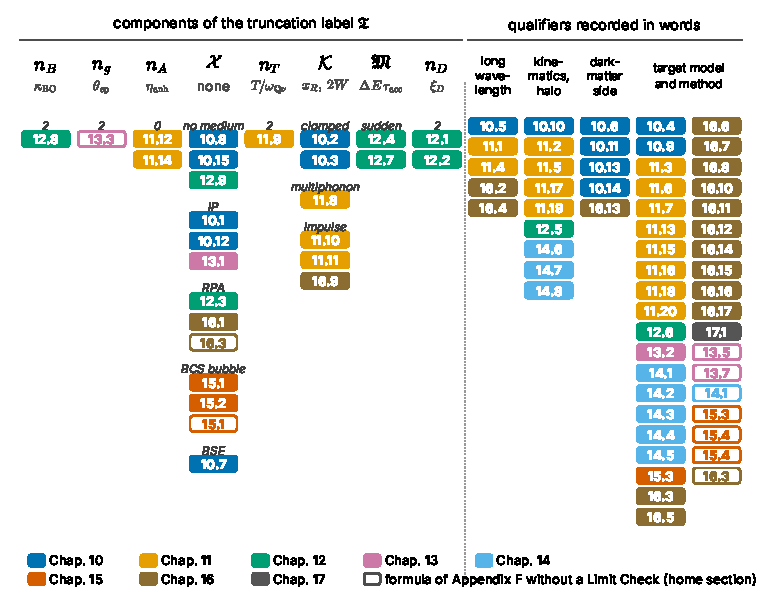
\includegraphics[width=\linewidth]{figures/ch09/fig9_3.pdf}
  \caption{The Limit Checks of \crefrange{chap:10}{chap:17} placed by the axis of their leading correction. Left: the eight components of the truncation label $\mathfrak{T}$, each with its small parameter (\cref{tab:8-params}); under each, the boxes whose comparison result lies one step from the formula along that component, grouped by the formula's value of that component, printed in italic (for example IP or impulse). Right: boxes whose leading correction is an expansion in a parameter that the label records only in words, sorted into four kinds. Filled chips: Limit Checks, colored by chapter. Hollow chips: formulas of \cref{tab:F-rows} without a box, labeled by the number of their home section, not of a box. The step of each box and its controlling parameter are listed in \cref{tab:9-limitchecks}.}
  \label{fig:9-axes}
\end{figure}

\Cref{fig:9-axes} places the 75 Limit Checks of \crefrange{chap:10}{chap:17} by the axis of their leading correction, and \cref{tab:9-limitchecks} lists each with its controlling parameter and its step. Twenty-five lie on a component of the label. Eleven are on the many-body axis. Among them are the crystal form-factor rate of \cref{sec:10.1}, which computes the rate of creating electron--hole pairs from independent-particle bands, and the Migdal rate through the loss function of \cref{sec:12.3}. The loss function of a superconductor in \cref{sec:15.1} is there too: its box compares the bare quasiparticle response with a conserving one, built so that it obeys charge conservation. Six are on the lattice regime, from the clamped lattice to the impulse limit, two on the anharmonic order, two on the Migdal regime, two on the multipole order, one on the thermal order and one on the Born--Oppenheimer order. Every Migdal scattering formula sits at $n_B = 2$, and the rate with phonon final states of \cref{sec:12.4} takes its next step there: the phonon energies in the electronic denominators give $2\langle\omega_{\mathrm{ph}}^2\rangle/\omega_e^2 = 2.9\times10^{-3}$ at the silicon gap, one step of $n_B$ in the counting of \cref{tab:8-params}. None of the boxes has its leading correction on $n_g$. The one formula whose next step is $n_g = 4$, the phonon-assisted electron-recoil rate of \cref{sec:13.3}, has no box, and its correction is the off-shell parameter $\theta_{\mathrm{ep}}$ of \cref{tab:8-params}.

The other 50 boxes expand in a qualifier: 5 in a long wavelength, 9 in the kinematics of the halo or the signal, 5 on the dark-matter side, and 31 in the model of the target. Two of the last are close to the label. Before any change of $\mathcal{X}$, the rate of the electron gas in \cref{sec:10.3} misses the gap and the interband peaks of the crystal, a change of target model. The band of \cref{sec:11.5} built from exact moments misses the skewness of the moment problem, not an anharmonic order. The split follows the chapters. In \cref{chap:12} seven of nine boxes lie on the label, in \cref{chap:10} seven of fifteen and in \cref{chap:11} six of twenty. In \cref{chap:14}, on magnetic excitations, none of the eight does, and in \cref{chap:16}, on novel targets such as Dirac materials, quantum dots and glasses, two of seventeen do. The label was built from the expansion of a crystal of electrons and nuclei in its small parameters, and the electronic, lattice and Migdal channels truncate along it. For the other targets the controlling parameter of the box is the target's own.

\begin{workedexample}{Three literature rates on the truncation label}\label{we:9-place}
We place three rates on $\mathfrak{T}$ and read from each placement the plot that its Limit Check draws. The rates are derived in \cref{sec:10.1,sec:10.2,sec:11.4}; here we use only their assumptions.

\emph{Crystal form-factor rate.} The electron-recoil rate of Essig and collaborators~\cite[Eqs.~(3.13) and (3.17)]{essig2016direct} squares the matrix elements of $\ee^{\ii\vect{q}\cdot\vect{r}}$ between Bloch states of independent electrons (\cref{chap:3}), with the valence bands filled at $T = 0$ and the nuclei clamped. Each assumption is a base value: no derivative coupling, no electron--phonon vertex, independent particles, no thermal occupation, and no multipole expansion, since the plane wave is kept whole. The rate sits at $\mathfrak{T}_0$, with the qualifier ``unscreened''. Every integer step costs a small parameter of \cref{tab:8-params}, and the many-body step costs an amount that no parameter predicts, so the many-body step is computed: IP to RPA to RPA with local fields. Screening is strongest at small $q$, where the long-range Coulomb field of the induced charge acts, and fades at large $q$. The controlling parameter is therefore the momentum transfer at fixed energy, and \cref{lim:10.1a} plots the rate weight against $q/q_0$, with $q_0 = \alpha m_e$, for the three approximations. The screened response is 0.05 of the unscreened one at the kinematic edge and 0.22 at $q_0$, and the $q$-integrated rate at \SI{5}{eV} is 0.47 of it. Nothing is shaded. The status follows: the formula is a definite point of the label, but its leading correction is of order one across the whole range, and \cref{sec:10.2} computes the rate with screening.

\emph{Loss-function rate.} The rate of Knapen and collaborators and of Hochberg and collaborators~\cites[Eqs.~(6) and (13)]{knapen2021dark}[Eq.~(1)]{hochberg2021determining} writes the response through the loss function $\Imag[-1/\varepsilon(\vect{q},\omega)]$. The identity \cref{eq:8.4-exact} makes this form exact for a coupling to the total charge at any lattice and for a coupling to the electron density with the nuclei clamped. The many-body axis is then not truncated by the formula; $\mathcal{X}$ is whatever approximation the loss function is computed in, RPA with local fields in the tables of \cref{sec:10.2}. The truncation is the clamped lattice, for a coupling to electrons alone. Releasing the nuclei is a step of the lattice regime, from no phonon in the final state to one phonon, and it adds the electron-following sector of \cref{sec:8.6}: the electrons that move with a nucleus carry an acoustic peak inside the phonon band. The controlling parameter is the energy deposit against the top of the phonon band, $\omega/\omega_{\max}$, and \cref{lim:10.2a} shades the energies above the band, where the two couplings share the formula. Below it, for dark matter of \SI{1}{MeV} and in a model of the acoustic peak, the electron-only coupling has more than $10^4$ times the rate that electronic excitations give at the same energies. The formula is established above the phonon band; inside it, for an electron-only coupling, the size of the correction rests on a model.

\emph{Free nuclear recoil.} The recoil rate of Lewin and Smith with the Helm form factor~\cite{lewin1996review}, \cref{eq:11.4-LS} with \cref{eq:2.2-helm}, assumes a nucleus that is free, at rest and recoils as a whole. In the label this is $\mathcal{K}$ = impulse at zero width, $n_B = 0$, the same placement as the elastic recoil of \cref{lim:1.3a}. The mean deposit $E_R$ is exact at every anharmonic and thermal order, since it is fixed by the sum rule \cref{eq:5.6-sum}. The leading correction is the next term of the impulse expansion, the Doppler width of the bound nucleus, of relative size $x_R^{-1/2}$. The controlling parameter is $x_R$, and \cref{lim:11.4a} plots the crystal rate over the free-recoil rate against it, with the multiphonon response of silicon as the fuller result and the Gaussian of the impulse approximation as the leading correction. For \SI{1}{GeV} dark matter the two agree within \SI{10}{\percent} for $x_R \ge 2.3$, at $q \ge \SI{70}{keV}$.

The two boxes on the impulse axis draw their bands at different values of one parameter. \Cref{lim:1.3a} asks of the spectrum at one momentum transfer that its rms width be below a third of $E_R$, which needs $x_R \ge 9$ for its oscillator. \Cref{lim:11.4a} asks of the rate at a given energy, which sums the response over momentum transfers with a smooth halo weight, that it agree within \SI{10}{\percent}. That is met at smaller $x_R$: with the mean deposit exact, the width changes such a sum only at second order. Where the band starts depends on the quantity compared and on the tolerance, and each caption states both.
\end{workedexample}

\subsection{The formal record of the limits}\label{sec:9.4-appF}

\Cref{tab:F-rows} of \cref{app:F} has one row for each formula that the book recovers as a limit, in the order of the chapters. For the channel chapters the appendix has 90 rows. Eighty belong to the 75 Limit Checks, since a box may compare two formulas in its panels. Ten have no box; they are marked so in the first column and appear as hollow chips in \cref{fig:9-axes}. Six of the 90 rows have an unsized leading correction, one that the book identifies but to which it assigns no number. A formula of this kind is established at its own point of $\mathfrak{T}$ and open beyond it; \cref{chap:22} collects the open items of the book, each with the missing step that would close it. To find a formula, a reader goes from the channel in \cref{tab:9-atlas} to its home section, and from there to its row in \cref{tab:F-rows}; \cref{tab:9-limitchecks} gives the same entry point by Limit Check.

% Generated by figscripts/ch09/fig9_3.py; do not edit by hand.
{\small
\setlength{\tabcolsep}{4pt}
\begin{longtable}{@{}>{\raggedright\arraybackslash}p{0.11\linewidth}>{\raggedright\arraybackslash}p{0.32\linewidth}>{\raggedright\arraybackslash}p{0.27\linewidth}>{\raggedright\arraybackslash}p{0.23\linewidth}@{}}
\caption{The Limit Checks of \crefrange{chap:10}{chap:17}, by chapter. Controlling parameter: the variable on the horizontal axis of the box. Leading correction: the component of the truncation label $\mathfrak{T}$ of \cref{eq:8.5-label} along which the comparison result lies one step from the formula, with the step; where the step is not along a component, the kind of qualifier it expands in. Formulas recovered as limits without a box are listed in \cref{tab:F-rows}.}\label{tab:9-limitchecks}\\
\toprule
Limit Check & Formula & Controlling parameter & Leading correction \\
\midrule
\endfirsthead
\toprule
Limit Check & Formula & Controlling parameter & Leading correction \\
\midrule
\endhead
\bottomrule
\endfoot
\multicolumn{4}{@{}l}{\emph{\Cref{chap:10}}} \\
\ref{lim:10.1a} & Crystal form-factor rate & momentum transfer $q/q_0$ at fixed $\omega$ & $\mathcal{X}$: IP $\to$ RPA + LF \\
\ref{lim:10.2a} & Loss-function rate & energy over the top of the phonon band & $\mathcal{K}$: clamped $\to$ one-phonon \\
\ref{lim:10.2b} & Sum-rule bounds on the loss function & momentum transfer $q$ & $\mathcal{K}$: clamped $\to$ one-phonon \\
\ref{lim:10.3a} & Lindhard and Mermin loss-function rates & energy over the gap, $\omega/\Eg$ & target model and method \\
\ref{lim:10.3b} & Plasmon production from the pole of $1/\varepsilon$ & momentum over the plasmon cutoff & long wavelength \\
\ref{lim:10.4a} & Crystal responses of the effective operators & current-row rate over density-row rate & dark-matter side and coupling \\
\ref{lim:10.5a} & Bethe--Salpeter exciton rate & momentum transfer $|\vect{q}|$ & $\mathcal{X}$: BSE, one time ordering $\to$ both \\
\ref{lim:10.7a} & Absorption with in-medium mixing & boson mass $m_\phi$ & $\mathcal{X}$: no medium $\to$ measured $\varepsilon$ \\
\ref{lim:10.7b} & Scalar absorption through the kinetic-energy row & upper cutoff of the spectral sum & target model and method \\
\ref{lim:10.8a} & Pair absorption & line width over the kinetic energy of the pair & kinematics and halo \\
\ref{lim:10.8b} & Dark Compton scattering & boson mass over electron mass & dark-matter side and coupling \\
\ref{lim:10.9a} & Inelastic electron recoil in crystals & mass splitting $\Delta_\chi$ & $\mathcal{X}$: IP $\to$ RPA + LF \\
\ref{lim:10.9b} & Boosted dark matter: the density row & dark-matter speed $v$ & dark-matter side and coupling \\
\ref{lim:10.9c} & Fermionic absorption on electrons & dark-matter mass over the binding energy & dark-matter side and coupling \\
\ref{lim:10.9d} & In-medium decay of an excited state & splitting over the valence plasma frequency & $\mathcal{X}$: no medium $\to$ measured $\varepsilon$ \\
\addlinespace
\multicolumn{4}{@{}l}{\emph{\Cref{chap:11}}} \\
\ref{lim:11.1a} & Long-wavelength acoustic structure factor & $q/q_{\mathrm{BZ}}$ & long wavelength \\
\ref{lim:11.1b} & Light-mediator single-phonon rate & dark-matter mass over the acoustic edge & kinematics and halo \\
\ref{lim:11.1c} & Sphere-averaged longitudinal speed & elastic anisotropy (Zener ratio) & target model and method \\
\ref{lim:11.2a} & Born-charge single-phonon rate & momentum transfer $q$ in three directions & long wavelength \\
\ref{lim:11.2b} & Polar matrix element and band integral & dark-matter mass $\mchi$ & kinematics and halo \\
\ref{lim:11.2c} & Static dielectric constant of one polar branch & share of one polar branch & target model and method \\
\ref{lim:11.2d} & Born charge over $\varepsilon_\infty$ from the LO--TO splitting & misfit of the inputs to the Lyddane--Sachs--Teller relation & target model and method \\
\ref{lim:11.3a} & Multiphonon incoherent approximation & $q/q_{\mathrm{BZ}}$ & $\mathcal{K}$: incoherent $\to$ coherent multiphonon \\
\ref{lim:11.3b} & Second-order thermal diffuse scattering & distance from a reciprocal-lattice vector & $n_T$: classical $\to$ quantum occupations \\
\ref{lim:11.4a} & Free nuclear recoil with the Helm form factor & recoil parameter $x_R$ & $\mathcal{K}$: impulse $\to$ multiphonon \\
\ref{lim:11.4b} & Fermionic absorption on nuclei & dark-matter mass $\mchi$ & $\mathcal{K}$: impulse $\to$ multiphonon \\
\ref{lim:11.5a} & Anharmonic corrections to multiphonon weights & momentum in units of the zero-point momentum & $n_A$: $0 \to 2$ \\
\ref{lim:11.5c} & The Markov--Krein band & threshold in standard deviations & target model and method \\
\ref{lim:11.5b} & Solid helium: quasi-harmonic and self-consistent phonons & Lindemann ratio & $n_A$: $0 \to$ all even orders \\
\ref{lim:11.6a} & Incoherent spin absorption & boson mass $m_\phi$ & target model and method \\
\ref{lim:11.6b} & Lifshitz mass-defect Green function & phonon frequency, at three mass defects & target model and method \\
\ref{lim:11.7a} & Daily modulation from the anisotropic response & momentum transfer $q$ & kinematics and halo \\
\ref{lim:11.8a} & Single-phonon absorption & boson mass $m_\phi$ near the polar phonon & target model and method \\
\ref{lim:11.8b} & Bulk acoustic resonator & quality factor of the mode over that of the halo field & kinematics and halo \\
\ref{lim:11.8c} & Resonant-mass drive of a scalar & frequency over the lowest mode of the body & target model and method \\
\addlinespace
\multicolumn{4}{@{}l}{\emph{\Cref{chap:12}}} \\
\ref{lim:12.2a} & Atomic Migdal effect at dipole order & multipole parameter $\xi_D$ & $n_D$: $2 \to$ all orders \\
\ref{lim:12.2b} & Migdal excitation of bound final states & multipole parameter $\xi_D$ & $n_D$: $2 \to$ all orders \\
\ref{lim:12.3a} & Crystal Migdal effect through the loss function & momentum given to the electrons, over $q_{\mathrm{BZ}}$ & $\mathcal{X}$: RPA $\to$ RPA + LF (diagonal) \\
\ref{lim:12.3b} & Crystal Migdal rate with free recoil & dark-matter mass (largest recoil energy) & $\mathfrak{M}$: sudden $\to$ moving nucleus \\
\ref{lim:12.3c} & Per-mass Migdal rate with the valence ionization factor & dark-matter mass $\mchi$ & kinematics and halo \\
\ref{lim:12.3d} & The Wannier picture of the boost & valence band width over the gap & target model and method \\
\ref{lim:12.4a} & Migdal effect with phonon final states & Doppler shift over the electronic energy & $\mathfrak{M}$: sudden $\to$ exact denominators \\
\ref{lim:12.4b} & Phonon-mediated Migdal effect & electronic energy against the phonon band & $n_B$: $2 \to 4$ \\
\ref{lim:12.6a} & Migdal-type absorption of a scalar & boson mass $m_\phi$ & $\mathcal{X}$: atomic $\to$ crystal loss function \\
\addlinespace
\multicolumn{4}{@{}l}{\emph{\Cref{chap:13}}} \\
\ref{lim:13.5a} & Phonon-assisted absorption as the optical limit & photon energy above the gap & $\mathcal{X}$: IP $\to$ BSE \\
\ref{lim:13.7a} & Zero-point renormalization by special displacements & supercell size & target model and method \\
\addlinespace
\multicolumn{4}{@{}l}{\emph{\Cref{chap:14}}} \\
\ref{lim:14.1a} & One-magnon rate at linear spin-wave order & inverse spin, $1/2|\vect{S}|$ & target model and method \\
\ref{lim:14.3a} & Absorption into magnons & applied over demagnetizing field; anisotropy over exchange & target model and method \\
\ref{lim:14.4a} & Data-driven spin response & orbital shift of the ion's $g$ factor & target model and method \\
\ref{lim:14.5a} & Chiral phonons and molecular magnets & dark-matter mass; level spacing over temperature & target model and method \\
\ref{lim:14.5b} & Multiferroic cross response & temperature over the ordering temperature & target model and method \\
\ref{lim:14.6a} & Transverse magnetization of a driven nuclear-spin ensemble & time over the coherence time of the field & kinematics and halo \\
\ref{lim:14.6b} & Gaussian-field signal and its power spectrum & record length over the coherence time & kinematics and halo \\
\ref{lim:14.6c} & Sensitivity scalings of the exponential-bin likelihood & record length over the coherence time & kinematics and halo \\
\addlinespace
\multicolumn{4}{@{}l}{\emph{\Cref{chap:15}}} \\
\ref{lim:15.1a} & Loss function of a superconductor near the pair-breaking edge & energy over the gap, on the kinematic edge & $\mathcal{X}$: bare BCS bubble $\to$ conserving \\
\ref{lim:15.2a} & Resummed loss function on the kinematic edge & energy over the gap, on the kinematic edge & $\mathcal{X}$: bare BCS bubble $\to$ conserving \\
\ref{lim:15.4a} & Phonon-assisted absorption: the normal-metal limit & energy over the gap & target model and method \\
\addlinespace
\multicolumn{4}{@{}l}{\emph{\Cref{chap:16}}} \\
\ref{lim:16.1a} & Background screening of Dirac-material rates & background dielectric constant & $\mathcal{X}$: Dirac bands $\to$ with remote bands \\
\ref{lim:16.2a} & One-dimensional plasmons of linear channels & momentum along the channel over $k_{\mathrm{F}}$ & long wavelength \\
\ref{lim:16.2b} & Acoustic plasmon of two components and its Landau width & plasmon speed over the Fermi speed of the light carriers & target model and method \\
\ref{lim:16.2c} & Effective medium of a layered stack & wave number times layer period & long wavelength \\
\ref{lim:16.3a} & Vacuum ejection with plane-wave final states & kinetic energy of the ejected electron & target model and method \\
\ref{lim:16.3b} & Quantum-dot rate and its bulk limit & energy above the dot gap, in confinement energies & target model and method \\
\ref{lim:16.4a} & Binned Frenkel rate & dark-matter mass $\mchi$ & target model and method \\
\ref{lim:16.5a} & Dopant absorption & donor density & target model and method \\
\ref{lim:16.6a} & Color-center creation and bond breaking & largest recoil energy over the threshold & $\mathcal{K}$: impulse $\to$ bound atom \\
\ref{lim:16.7a} & Two-level response to a classical strain or field & temperature & target model and method \\
\ref{lim:16.7b} & Dark-photon absorption on two-level systems & boson mass $m_\phi$ & target model and method \\
\ref{lim:16.7d} & Glass absorption below the Ioffe--Regel frequency & boson mass against the Ioffe--Regel frequency & target model and method \\
\ref{lim:16.7c} & Random media and the Born limit & medium potential over the dark-matter energy & dark-matter side and coupling \\
\ref{lim:16.8a} & Two-level relaxation by phonons and electrons & splitting over temperature; coupling to the electrons & target model and method \\
\ref{lim:16.8b} & The ohmic scaling limit & dimensionless ohmic coupling & target model and method \\
\ref{lim:16.8c} & Hopping and tunneling through one barrier & temperature over the tunneling crossover & target model and method \\
\ref{lim:16.8d} & Heat release of a cooled glass & time after cooling & target model and method \\
\addlinespace
\multicolumn{4}{@{}l}{\emph{\Cref{chap:17}}} \\
\ref{lim:17.5a} & Partial f-sum of the valence electrons & upper limit of the $f$-sum integral & target model and method \\
\end{longtable}
}

